\section{Resolution Benchmark}\label{sub:resolution}

The smoothing length is determined by the number of SPH particles in a region of the computational domain, which in turn defines the simulation's resolution in that region, see \cref{sub:gadget2}. The latter is small in high-density regions and large in low-density regions. To correctly account for the influence of gas drag on the inner binary, the smoothing length of the particles interacting with it must be considerably smaller than the binary's size. In my simulations, $N=50000$ is used. \cref{fig:resolution} shows that the present resolution is insufficient to capture the influence of gas drag.

In \cref{fig:resolution}, I present a snapshot at $t \approx 8$ yr, where the mass transfer is maximum. The x-axis represents the distance of each particle from the tertiary's center, while the y-axis represents the smoothing length of each particle. The horizontal yellow line corresponds to the orbital separation of the inner binary components, i.e. the binary's size. Finally the red area represents an approximation of the inner binary's close vicinity. More specifically, it corresponds to the position of the inner binary's center of mass $\pm$ the binary's size.
\begin{figure}[!htb]
    \centering
    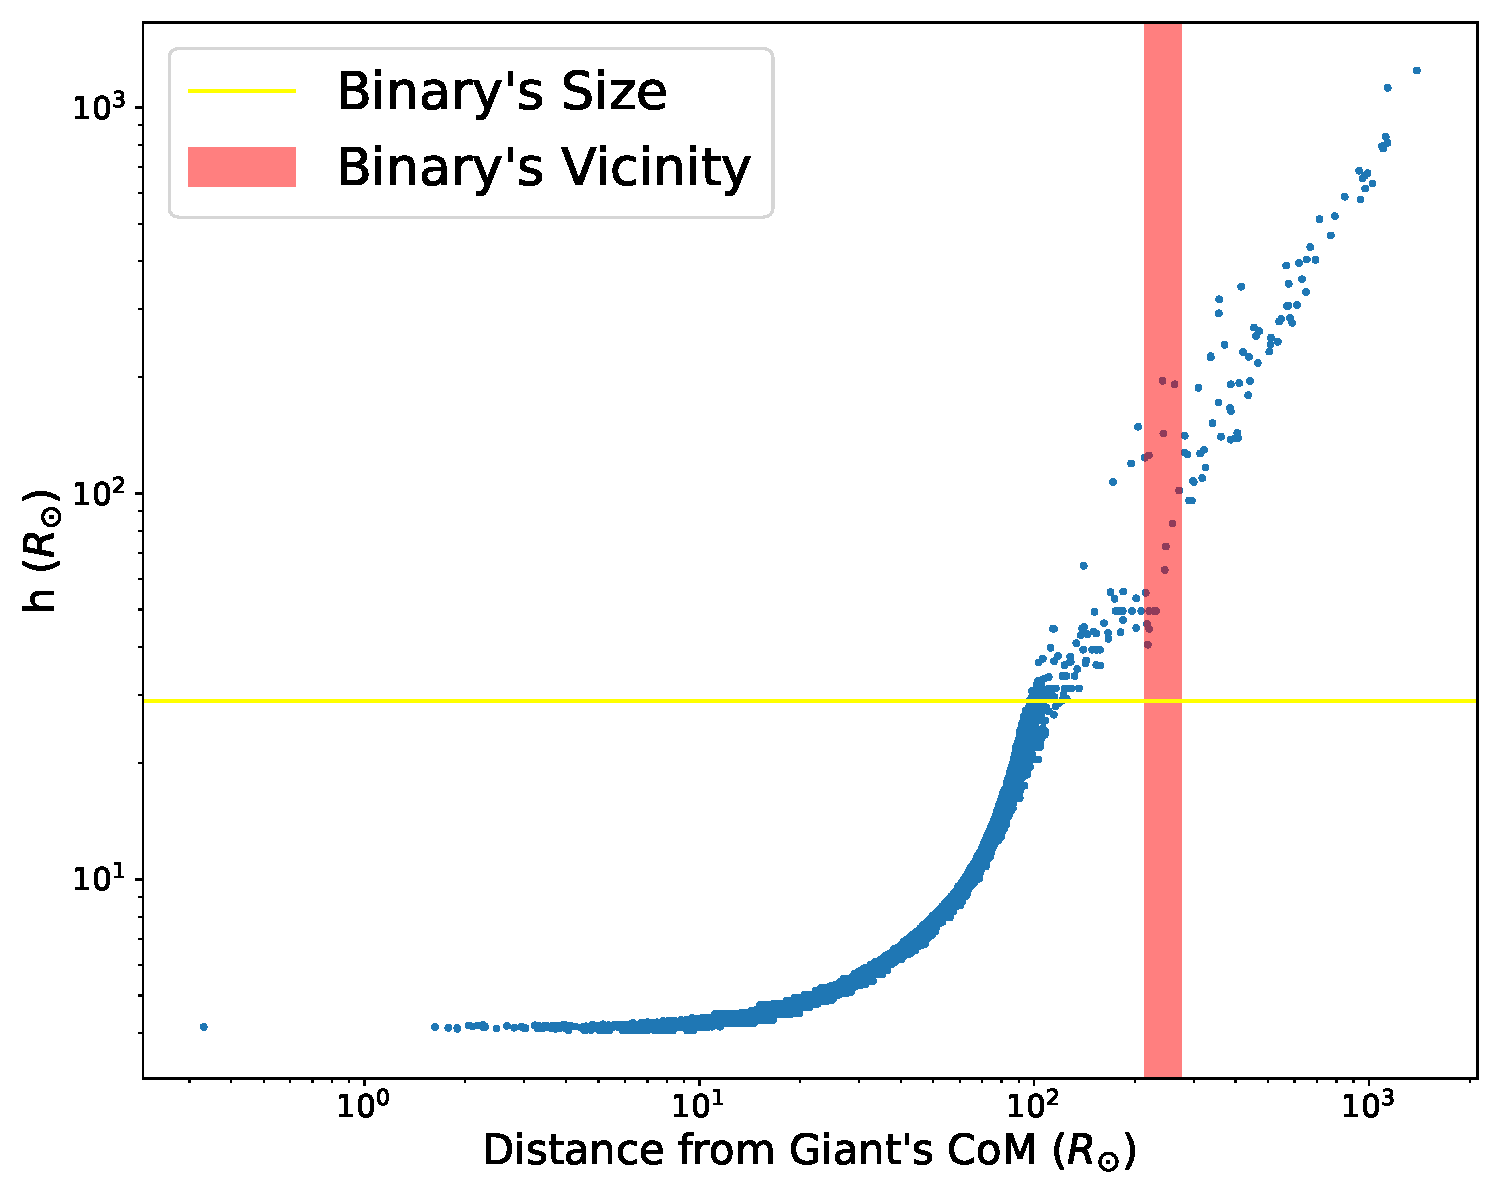
\includegraphics[width=0.9\textwidth]{Thesis/graphs/resolution_benchmark.pdf}
    \caption{Particles smoothing length in comparison to the binary's size at $t \approx 8$ yr, where the mass transfer is maximum.}
    \label{fig:resolution}
\end{figure}
Particles with smoothing lengths smaller than the binary's size, blue points bellow the yellow line, and close to the binary, blue point close/inside the red region, can influence hydrodynamically the inner orbit. At the current resolution, even when the mass transfer is maximum, the number of particles interacting with the binary is small (low-density mass stream), and thus their smoothing length is much larger than the size of the inner orbit. In conclusion, higher resolution simulations are required to safely estimate the evolution of the semi-major axis of the inner orbit.

Despite the fact that $N=50000$ is sufficient to initially resolve the giant at the moment of RLOF, see \cref{sec:1D_to_3D}, it is insufficient to accurately capture the gas drag on to the inner orbit. The fact that \cite{de2014evolution} use also $N=50000$ to examine mass transfer via RLOF by the outer star on the same system, was a motivation behind this particular choice. In their study, they employ a different SPH code. Nevertheless, both codes define the particles smoothing length in a similar fashion, thus it is a surprise that they are able to account for gas drag at seemingly the same resolution. 

To achieve higher resolution, I could simply increase the number of particles in my simulation. This is pretty straight forward in my code, however time restrictions require me to consider leaving this for future work. More specifically, with the available computational resources I obtain eight years of simulation in approximately five weeks of computational run time. Considering that the CPU time scales with the number of SPH particles as $NlogN$, increasing the number of particles by a factor of 5  results in several months of computational run time. 

In conclusion, with the current number of SPH particles the resolution of my simulations is insufficient to accurately capture the influence of the gas drag on the inner orbit. As a result, the gas drag is underestimated, while the models capture the gravitational interactions between the inner binary, the core of the tertiary, and its gaseous envelope. Regardless, I can still extract useful information about the evolution of the outer orbit and conjecture about the evolution of the inner orbit. 